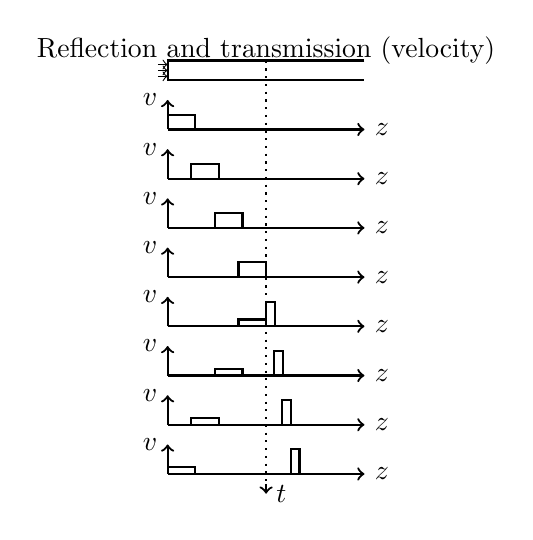
\begin{tikzpicture}[scale=0.25]

    \node at (5, 1.5) {Reflection and transmission (velocity)};

    \draw[black, thick] (10, 1) -- (0, 1) -- (0,0) -- (10, 0);

    %Schraffur
    %\fill[pattern={Dots[angle=45, distance={2pt}]}] (0, 0) rectangle (5, 1);
    %\fill[pattern={Dots[angle=45, distance={4pt}]}] (5, 0) rectangle (10, 1);
    
    \draw[->] (-0.5, 0.8) -- (0, 0.8);
    \draw[->] (-0.5, 0.5) -- (0, 0.5);
    \draw[->] (-0.5, 0.2) -- (0, 0.2);

    \draw[black, thick, dotted] (5, 1) -- (5, -20.5);
    \draw[->, thick] (5, -20.5) -- (5, -21) node[right] {$t$};

    %Diagramm 1:
    \draw[->, thick] (0, -2.5) -- (0, -1.0) node[left] {$v$};
    \draw[->, thick] (0, -2.5) -- (10, -2.5) node[right] {$z$};
    \draw[thick] (0, -1.75) -- (1.4, -1.75) -- (1.4, -2.5);

    %Diagramm 2:
    \draw[->, thick] (0, -5) -- (0, -3.5) node[left] {$v$};
    \draw[->, thick] (0, -5) -- (10, -5) node[right] {$z$};
    \draw[thick] (1.2, -5) -- (1.2, -4.25) -- (2.6, -4.25) -- (2.6, -5);

    %Diagramm 3:
    \draw[->, thick] (0, -7.5) -- (0, -6) node[left] {$v$};
    \draw[->, thick] (0, -7.5) -- (10, -7.5) node[right] {$z$};
    \draw[thick] (2.4, -7.5) -- (2.4, -6.75) -- (3.8, -6.75) -- (3.8, -7.5);

    %Diagramm 4:
    \draw[->, thick] (0, -10) -- (0, -8.5) node[left] {$v$};
    \draw[->, thick] (0, -10) -- (10, -10) node[right] {$z$};
    \draw[thick] (3.6, -10) -- (3.6, -9.25) -- (5, -9.25) -- (5, -10);

    %Diagramm 5:
    \draw[->, thick] (0, -12.5) -- (0, -11) node[left] {$v$};
    \draw[->, thick] (0, -12.5) -- (10, -12.5) node[right] {$z$};
    \draw[thick] (3.6, -12.5) -- (3.6, -12.15) -- (5, -12.15) -- (5, -12.5);
    \draw[thick] (5, -12.5) -- (5, -11.25) -- (5.45, -11.25) -- (5.45, -12.5);

    %Diagramm 6:
    \draw[->, thick] (0, -15) -- (0, -13.5) node[left] {$v$};
    \draw[->, thick] (0, -15) -- (10, -15) node[right] {$z$};
    \draw[thick] (2.4, -15) -- (2.4, -14.65) -- (3.8, -14.65) -- (3.8, -15);
    \draw[thick] (5.4, -15) -- (5.4, -13.75) -- (5.85, -13.75) -- (5.85, -15);

    %Diagramm 7:
    \draw[->, thick] (0, -17.5) -- (0, -16) node[left] {$v$};
    \draw[->, thick] (0, -17.5) -- (10, -17.5) node[right] {$z$};
    \draw[thick] (1.2, -17.5) -- (1.2, -17.15) -- (2.6, -17.15) -- (2.6, -17.5);
    \draw[thick] (5.8, -17.5) -- (5.8, -16.25) -- (6.25, -16.25) -- (6.25, -17.5);

    %Diagramm 8:
    \draw[->, thick] (0, -20) -- (0, -18.5) node[left] {$v$};
    \draw[->, thick] (0, -20) -- (10, -20) node[right] {$z$};
    \draw[thick] (0, -19.65) -- (1.4, -19.65) -- (1.4, -20);
    \draw[thick] (6.25, -20) -- (6.25, -18.75) -- (6.7, -18.75) -- (6.7, -20);


\end{tikzpicture}
